\documentclass[a4paper,10.5pt,twocolumn]{jsarticle}
\usepackage{eshouroku}
\usepackage[dvipdfmx]{graphicx}
\usepackage{amsmath}
\usepackage{url}
\usepackage{here}
\usepackage{booktabs}
\usepackage{remreset}
\usepackage{pdfpages}
\usepackage{comment}

\makeatletter
	\renewcommand{\theequation}{% 式番号の付け方
	\thesection\arabic{equation}}
	\@addtoreset{equation}{section}

	\renewcommand{\thefigure}{% 図番号の付け方
	\thesection\arabic{figure}}
	\@addtoreset{figure}{section}

	\renewcommand{\thetable}{% 表番号の付け方
	\thesection\arabic{table}}
	\@addtoreset{table}{section}
\makeatother
%\numberwithin{equation}{section}
%\numberwithin{table}{section}
%\numberwithin{figure}{section}


\boldmaintrue% 主文を太字にするモード(指導教員添削時はこちら)
%\boldmainfalse% 主文を普通文字にするモード(抄録印刷時はこちら)
\graphicspath{{./figs/}}
\begin{document}
\twocolumn[
 \講演番号{B-XX}% 必要ない場合には書かない
 \日本語タイトル{\huge}{神経免疫相互作用に着想を得た\\マルチエージェントシステム型ニューラルネットワークの提案}
 \英語タイトル{\large}{Proposal of Neural Network composed of Multi-Agent System Inspired by Nervous-Immune Interaction}
 \筆者一名{5335}{柚木開登}

 \指導教員一名{山本哲也}
 %\指導教員二名{東京花子}{京都紀夫}
 %\指導教員なし
]

%\addcontentsline{toc}{section}{\refname}% 追加

\graphicspath{{./figs/}} % 図が特定のフォルダにある場合には設定

\section{本研究の意義・目的}
\begin{comment}
本来的に大規模な計算資源を必要とするニューラルネットワークが
今日, あらゆる産業へ導入されるに至ったのは, クラウドコンピューティングの貢献がある.
一方で, 同市場拡大に伴って
プラットフォーマによる市場寡占, データセンターでの電力消費, データプライバシーの課題が表面化した.
こうしたクラウドの課題克服に向けて, 
データを集約せずにネットワークの端点(エッジ)で処理するエッジコンピューティングが注目
されている.
\end{comment}
エッジコンピューティングでの機械学習手法として連合学習(Federareted Lerning)が提案されている.
連合学習では, 学習データを集約せずネットワーク中の各ノードで学習し, 
その結果得たパラメータ差分のみを通信することによって
大規模な学習済みモデルを構築するため, プライバシーを含んだ学習データは保護される.
機械学習への期待と世界的な個人情報保護の動きの高まりから, 
将来的に連合学習は情報社会において重要な位置を占めることが予測される.

一方, 連合学習の実用化に際しては, 
従来, データセンターで動いていたモデルを計算資源に乏しいエッジ環境に投入する必要があることから
少なくとも以下2点の課題が考えられる.
1つ目は学習パラメータ削減によるモデルの軽量化, 
2つ目は, エッジ環境内の不均一計算資源の最大限の有効利用
である.
前者については刈り込みや, ニューラルアーキテクチャ探索, 後者についてはエージェント志向アーキテクチャによる
分散処理システムや遊休計算資源を用いた大規模分散計算等があり, 
今日までに多様な先行事例・研究が成されている. 
両者を満たしたモデルを構築できれば, 
大規模なニューラルネットワークのエッジ環境への投入を可能にし, 
かつ環境内の計算資源の利用率を最大化することが期待できるが,  
両者を満たしたモデルに関する研究は著者の知る限り存在しない.

そこで本研究では, 将来的に導入が予測されるエッジコンピューティングアーキテクチャ及び, 
それに対応した機械学習手法である連合学習に向けて, 
自律分散性を持ったニューラルネットワークのパラメータ削減を提案する(\wfig{Method}).
\begin{figure}[H]
  \centering
  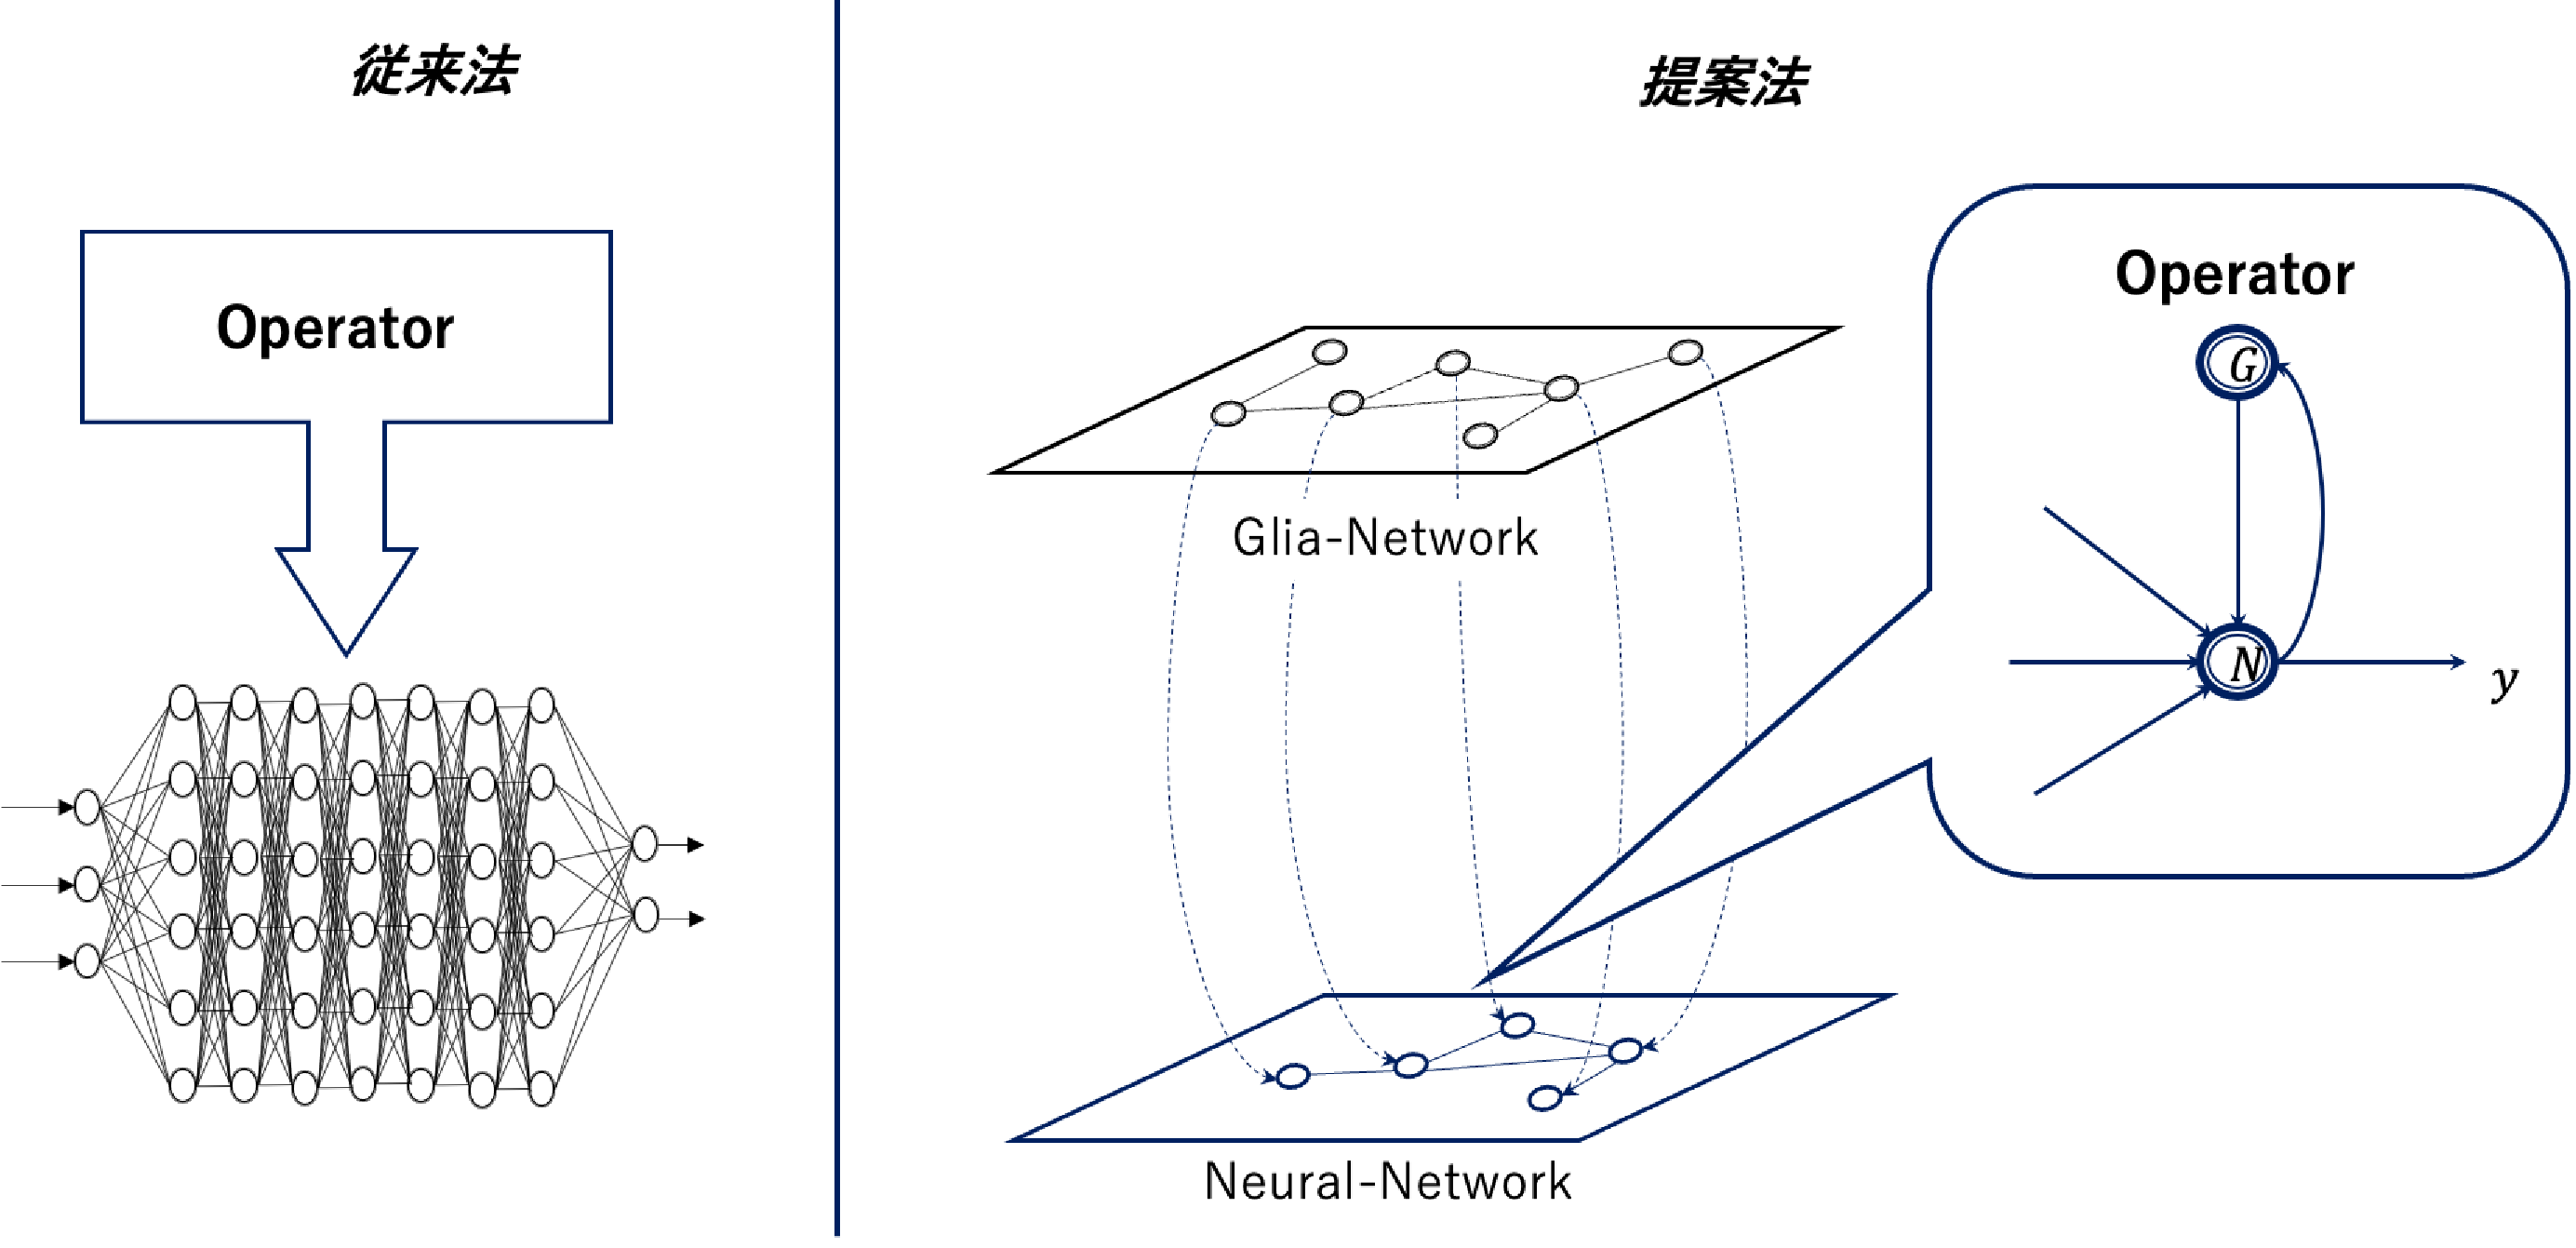
\includegraphics[width=8cm]{Method.pdf}
  \caption{従来法と提案法との比較}
  \label{fig:Method}
\end{figure}
\section{生物学的背景}
\subsection{神経免疫相互作用}
神経系と免疫系は独立したシステムではなく相互に調節を行い, 人体の恒常性を維持している
ことが知られている.
これは神経免疫相互作用(Neuroimmanue Interaction)と呼ばれ, 
古くから経験的に知られていたストレスと疾患の関係の医学的な証左である.
殊に脳内においては神経系をニューロン, 免疫系をミクログリアと呼ばれる中枢神経系グリア細胞が司っており, 
グリア--ニューロン間においても神経免疫相互作用が認められている\cite{Neuron-Glia}.

またミクログリアは, 脳の発達において重要な役割を果たす
シナプスの刈り込みを担当する.
特に, 霊長類の大脳皮質では
生後直後からシナプス数が急速に増大し, 小児期に最大値に達したのち, 
刈り込みが行われ減少していくオーバーシュート型シナプス形成と呼ばれる特徴的なシナプスリモデリングが行われる.
このシナプス形成の刈り込み段階において, 
統合失調症では通常よりも多く行われ, ASDでは通常よりも少なく行われることが
確認されており, シナプスの刈り込みが脳の高次機能の維持・発現の要因である可能性が示唆される。
\subsection{グリアアセンブリ}
\label{sec:g-asem}
生体の脳は神経細胞とグリア細胞によって構成される.
グリア細胞とは脳内細胞のうち神経細胞以外を指し, 
ミクログリア(microglia), アストロサイト(astrocyte),
オリゴデンドロサイト(oligodendrocyte)の三種が大多数を占める.
グリア細胞の役割は神経細胞への栄養運搬, 血流の制御, 電気信号の速度制御, 免疫等
多岐にわたるが, 巨大なグリア細胞同士のネットワーク 
---グリアアセンブリ(Glia Assembly)--- 
が確認されており, 異種グリア細胞が互いに協調し合いながら, 
脳の機能維持を行っているものの, 
その具体的なメカニズムは現在までに知られていない.
\section{提案モデル}
\subsection{概要}
本モデルは, 自律分散的なパラメータ削減として生体の脳で行われるグリア細胞による
シナプスの刈り込みをモデル化し, マルチエージェントシステムとして実装している.
投入するエージェントはNeuro-Agent, Synapse-Agent, Glia-Agentであり, 
それぞれがニューロン, シナプス, グリア細胞に対応する. 
また神経免疫相互作用に着想を得て, 


\subsection{神経免疫相互作用に基づくフィードバック}
これらのうち, 特に$NA$と$GA$の相互制御に関わる部分を詳しく述べる.
双方の制御は以下の手順で行われる.

GAからNAへの制御はNAに接続された最も重みの小さなシナプスとの接合を切る.
\subsection{グリアネットワーク}
\wsec{g-asem}節に述べた通り, 実際の脳ではミクログリアは単体で
刈り込みを行っているのではなく, 
グリアアセンブリを介して, 協調し全体としての利益に資する行動を
とっているものと見られる.

本研究ではグリアアセンブリの模倣として$GA$同士のネットワークである
グリアネットワークを定義した.
グリアネットワークの役割は, 時空間的に
局所的な刈り込みが行われネットワークの破綻を防ぐというものである.

このアイデアは抑制信号を伝達するという形で実装した.
抑制信号は, グリアネットワーク上の伝播距離(ホップ数)に応じて減衰していく.
本実験では単純にホップカウントに0.1を乗じた値だけ減少するように実装した.
なお, 複数の距離が与えられた場合, 最も近い$GA$の影響を優先する.
\wfig{GliaNetworks}の$g_2$の場合, 
$g_0\rightarrow g_1\rightarrow g_2$と$g_0\rightarrow g_2$の経路では後者の経路のみを考えることになる.

\begin{figure}[H]
  \centering
  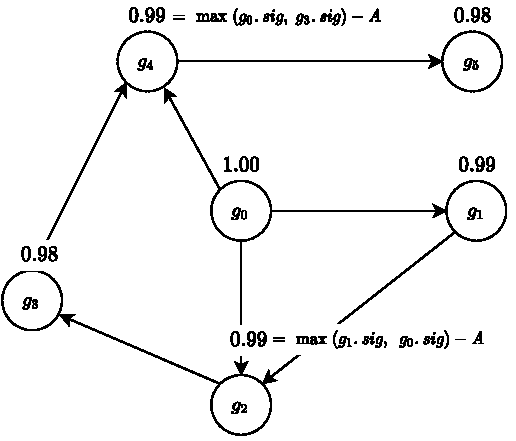
\includegraphics[width=6cm]{GliaNetworks.pdf}
  \caption{グリアネットワークでの抑制信号の伝達}
  \label{fig:GliaNetworks}
\end{figure}
\section{計算機実験}
学習タスクは, 6bitの入力の上位3bitのいずれかに1が入っているかどうか
の判別である. 出力値は結果が真である確率である. 
その他のパラメータは以下に示す通りである(\wtab{param}).
\begin{table}[H]
  \caption{パラメータ一覧}
  \label{tab:param}
  \centering
   \begin{tabular}{ll}
    \toprule
      パラメータ&値\\\midrule\midrule
      学習率$\eta$&$0.01$\\
      エポック数$Epocs$&$500$\\
      ミニバッチサイズ$miniBatchSize$&$100$\\
      初期ニューロン数$Neurons$&$31$\\
      初期グリア数$Glias$&$31$\\
      初期シナプス数$Mill$&$182$\\
      入力サイズ$Inputs$&$6$\\
      出力サイズ$Outputs$&$1$\\
    \bottomrule
   \end{tabular}
 \end{table}
計算機実験の結果, \wfig{syna}が\wfig{span}得られた.


 
\section{結論}
グリア細胞に着想を得た監視エージェントを導入することによって
全体の管理者のいないMASに対応した
ニューラルネットワークの学習パラメータの削減を行うことができた.
このパラメータの削減にあたっては, 学習精度の悪化が認められなかったことから, 
刈り込みが適切に行われたものと評価できる
一方で, グリアネットワークの構造依存性や
MASに特有な問題(合意制御, 環境認識), あるいは畳み込みのMAS化など
実用化にあたっては
さらなる発展が必要である.
\begin{align}
  \exp(x) exp(x)
\end{align}
 \begin{thebibliography}{99}
  \bibitem{Neuron-Glia} 	
野村靖幸,北海道大学,神経免疫相関とくにニューロン・グリア相互作用機構に関する分子薬理学的研究, \url{https://kaken.nii.ac.jp/ja/grant/KAKENHI-PROJECT-06454595/}
  \bibitem{Tensorizing}
  Novikov, Alexander, et al. "Tensorizing neural networks." Advances in neural information processing systems 28 (2015).
  \bibitem{次数重み付き平均法}
  原田和明, 右田剛史, and 高橋規一.``ニューラルネットワークの分散学習における新たな合意重み決定法.'' IEICE Conferences Archives. The Institute of Electronics, Information and Communication Engineers, 2019.
\end{thebibliography}
 \end{document}
